% Created 2016-05-01 Sun 21:54
\documentclass[11pt]{article}
\usepackage[utf8]{inputenc}
\usepackage[T1]{fontenc}
\usepackage{fixltx2e}
\usepackage{graphicx}
\usepackage{grffile}
\usepackage{longtable}
\usepackage{wrapfig}
\usepackage{rotating}
\usepackage[normalem]{ulem}
\usepackage{amsmath}
\usepackage{textcomp}
\usepackage{amssymb}
\usepackage{capt-of}
\usepackage{hyperref}
\usepackage[portuguese, ]{babel}
\author{André Peric Tavares, Giulio Parva Denardi}
\date{\today}
\title{Projeto de Compiladores\\\medskip
\large Trabalho para a disciplina Compiladores na Universidade Federal do ABC sob orientação da Profa. Mirtha Lina Fernández Venero}
\hypersetup{
 pdfauthor={André Peric Tavares, Giulio Parva Denardi},
 pdftitle={Projeto de Compiladores},
 pdfkeywords={},
 pdfsubject={},
 pdfcreator={Emacs 24.5.1 (Org mode 8.3.3)}, 
 pdflang={Pt-Br}}
\begin{document}

\maketitle
\tableofcontents


\section{Introdução}
\label{sec:orgheadline1}
\textbf{negrito}
\emph{itálico}
\href{https://google.com}{google}
\hyperref[sec:orgheadline1]{link}
imagem:
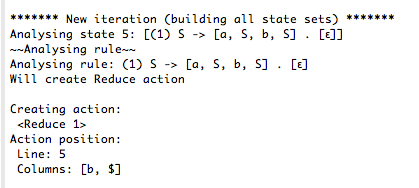
\includegraphics[width=.9\linewidth]{./media/Screenshot 2016-04-25 17.54.18.png}

\section{Objetivos}
\label{sec:orgheadline2}
O objetivo é criar um programa que, dada uma gramática de entrada,
produza e apresente passo-a-passo o cálculo dos conjuntos FIRST e FOLLOW e da
construção das tabelas LL e LR.
\section{Justificativa}
\label{sec:orgheadline4}
Existem diversas ferramentas que geram as tabelas, mas geralmente os passos são
omitidos ou o código é muito complexo. Neste projeto, tentamos ao mesmo tempo
apresentar na saída do programa cada etapa do processo e manter o código
legível e simples, mesmo quando isso significar ser menos eficiente. Deste modo,
o programa beneficia aqueles que estão estudando os conceitos teóricos e também
é de fácil entendimento àqueles que desejam estendê-lo.

Além disso, justificamos várias decisões do ponto de vista de Engenharia de
Software em \ref{sec:orgheadline3}, apresentando na
prática como várias boas práticas de programação podem ser aplicadas.

\section{Metodologia}
\label{sec:orgheadline5}
Decidimos utilizar a linguagem Java para a implementação, especialmente pelo
fato de ser estática (o que previne muitos \emph{bugs} na fase de compilação),
orientada a objetos (fazendo com que seja possível abstrair muitos conceitos em
classes, tornando o código organizado e simples de entender) e popular.

O código do projeto está disponível na pasta \texttt{sources}. Além disso, a versão
mais atual pode ser encontrada em \url{https://github.com/ufabcompiladores/projetofinal}.

Utilizamos o Spring Framework (\url{https://spring.io/}). Assim, o \emph{front end} é
\emph{web}, podendo ser acessado de qualquer navegador.

\section{Funcionamento}
\label{sec:orgheadline14}
\subsection{Produção de cadeia vazia}
\label{sec:orgheadline6}
O cálculo dos conjuntos FIRST e FOLLOW exigem em diversos momentos saber se
um determinado não terminal produz \(\epsilon\). Por exemplo, considere a sequência
de símbolos \emph{ABC}. Queremos calcular FIRST(ABC). Sabemos que

\begin{center}
FIRST(ABC) = FIRST(A) \(\oplus\) FIRST(BCD)
\end{center}

e o resultado desta operação é somente FIRST(A) se \(A\) não produz \(\epsilon\) ou
FIRST(A) - \(\epsilon\) se \(\epsilon\) \(\in\) FIRST(A). Então é conveniente saber de
antemão quais símbolos produzem \(\epsilon\).

Para tanto, usa-se o método \texttt{buildAllNonTerminalsThatProduceEps} na classe
\texttt{Grammar}. O algoritmo utilizado é simples: primeiro, verifica-se todos os não
terminais que produzem diretamente \(\epsilon\), isto é, aqueles que têm uma regra
que produz \(\epsilon\) sem etapas intermediárias, como em \(A \rightarrow \epsilon\).

Em seguida, todas as regras são percorridas, e se todos os símbolos da parte
direita de uma regra produzem \(\epsilon\), então adicionamos o produtor dessa regra
à lista de não terminais que produzem \(\epsilon\). Todas as regras são percorridas
novamente até que nenhum símbolo novo tenha sido adicionado à lista de símbolos
que produzem \(\epsilon\). Em outras palavras, até que o ponto fixo seja atingido.

Por exemplo, considere a seguinte gramática:

\begin{center}
A \(\rightarrow\) BC \\
B \(\rightarrow\) \(\epsilon\) \\
C \(\rightarrow\) \(\epsilon\)
\end{center}

A tabela a seguir mostra o resultado desse algoritmo aplicado à gramática
anterior em cada iteração.

\begin{center}
\begin{tabular}{llll}
Produz \(\epsilon\)? & A & B & C\\
Iteração 1 & não & sim & sim\\
Iteração 2 & sim & sim & sim\\
Iteração 3 & sim & sim & sim\\
\end{tabular}
\end{center}

Na iteração 3, o conjunto de elementos que produzem \(\epsilon\) não mudou, e assim
o algoritmo termina.

O código é apresentado a seguir.

\begin{verbatim}
private final void buildAllNonTerminalsThatProduceEps() {
  Set<Symbol> nonTerminalsThatGenerateEps = new HashSet<Symbol>();

  // rules that directly generate eps
  for (Symbol nonTerminal : nonTerminals) {
    for (Rule rule : rules.get(nonTerminal)) {
      if (rule.producesEmptyString()) {
        nonTerminalsThatGenerateEps.add(nonTerminal);
      }
    }
  }

  // iterates until fp is found
  boolean newNonTerminalThatGeneratesEpsHasBeenFound = true;
  while (newNonTerminalThatGeneratesEpsHasBeenFound) {
    newNonTerminalThatGeneratesEpsHasBeenFound = false;
    int setSizeBeforeIteration = nonTerminalsThatGenerateEps.size();

    for (Symbol nonTerminal : nonTerminals) {
      for (Rule rule : rules.get(nonTerminal)) {
        // verifies if all symbols from rule produce eps
        List<Symbol> production = rule.getProduction();
        boolean allSymbolsFromProductionProduceEps;
        allSymbolsFromProductionProduceEps = production
            .stream()
            .allMatch(symbol -> nonTerminalsThatGenerateEps.contains(symbol));

        // if so, add it to set
        if (allSymbolsFromProductionProduceEps) {
          nonTerminalsThatGenerateEps.add(nonTerminal);
        }
      }
    }

    // verifies whether some non terminal has been added to set
    int setSizeAfterIteration = nonTerminalsThatGenerateEps.size();
    if (setSizeBeforeIteration != setSizeAfterIteration) {
      newNonTerminalThatGeneratesEpsHasBeenFound = true;
    }
  }

  // initialise Map
  Map<Symbol, Boolean> producesEps = new HashMap<Symbol, Boolean>();
  for (Symbol nonTerminal : nonTerminals) {
    producesEps.put(nonTerminal, nonTerminalsThatGenerateEps.contains(nonTerminal));
  }
  for (Symbol terminal : terminals) {
    producesEps.put(terminal, false);
  }

  this.nonTerminalsToProducesEps = producesEps;
}
\end{verbatim}

\subsection{Representação dos conjuntos FIRST e FOLLOW}
\label{sec:orgheadline7}
Uma das principais funcionalidades do programa deste trabalho é não só calcular
os conjuntos FIRST e FOLLOW, mas fazer isso apresentando as etapas
intermediárias, fazendo com que o usuário veja cada passo do algoritmo. Isso faz
com que o cálculo desses conjuntos não seja o mais eficiente possível, pois
precisamos lidar também com o \emph{output} sem pular nenhuma etapa.

Para isto, criamos classes \texttt{First} e \texttt{Follow}. Estas classes têm atributos que
indicam a \emph{representação} do conjunto dado em termos de outros conjuntos.

Por exemplo, considere os seguintes atributos da classe \texttt{Follow}:

\begin{verbatim}
private Set<Symbol> firstSets;
private Set<Symbol> firstSetsWithoutEps;
private Set<Symbol> followSets;
private Set<Symbol> terminals;
private boolean hasEOF;
\end{verbatim}

Suponha que um objeto dessa classe tenha as seguintes atribuições (aqui em
notação de teoria dos conjuntos):

\begin{center}
firstSets = \{A\} \\
firstSetsWithoutEps = \{B, C\} \\
followSets = \{D\} \\
terminals = \{a, b\} \\
hasEOF = true \\
\end{center}

Então esse conjunto seria

\begin{center}
FIRST(A) \(\cup\) (FIRST(B) - \(\epsilon\)) \(\cup\) (FIRST(C) - \(\epsilon\)) \(\cup\) FOLLOW(D)
\(\cup\) \{a\} \(\cup\) \{b\} \(\cup\) \{\$\}
\end{center}

Ambas as classes têm o método \texttt{toString} sobrescrito para exibir essa
representação como mostrado acima e um método \texttt{getAllElements} que coleta
todos os elementos vindos da união dos conjuntos.

\subsection{Cálculo dos conjuntos FIRST e FOLLOW}
\label{sec:orgheadline8}
De maneira semelhante à computação de todos os não terminais que geram \(\epsilon\),
o cálculo dos conjuntos FIRST e FOLLOW consiste, em essência, em iterar até
encontrar um ponto fixo.

Note que a aplicação direta da definição de FIRST e FOLLOW não funciona, pois
ela falharia no caso de definições recursivas que são dependentes entre
si. Por exemplo, considere o caso em que FIRST(A) = FIRST(B) e FIRST(B) =
FIRST(A). Para calcular FIRST(A), calcula-se FIRST(B). Mas FIRST(B) é FIRST(A),
o que resulta num \emph{loop} infinito. Em vez disso, começamos com todos os
conjuntos FIRST setados para \(\emptyset\), e a cada iteração atualizamos todos os
conjuntos até atingir um ponto fixo. 

O código a seguir mostra a implementação desse algoritmo para o cálculo dos
conjuntos FIRST.

\begin{verbatim}
public final void buildAllFirstSets() {

  // Initialize set
  // omitido

  // Get description of each first set
  Map<Symbol, First> firstSetDescriptions = buildAllFirstSetDescriptions();

  // Iterate until fixed point is found
  boolean someFirstSetHasChanged = true;
  while (someFirstSetHasChanged) {
    StringBuilder iterationSb = new StringBuilder();
    iterationSb.append("New iteration (building first sets)\n");
    someFirstSetHasChanged = false;

    // Copy elements from old first sets to new first sets
    // omitido

    // Updates, possibly getting new elements
    for (Symbol nonTerminal: nonTerminals){
      iterationSb.append(String.format("Updating First(%s)\n", nonTerminal));
      First firstDescription = firstSetDescriptions.get(nonTerminal);
      iterationSb.append(String.format("First(%s) = %s\n", nonTerminal, firstDescription));
      int numElementsBefore = firstSetsBeforeIteration.get(nonTerminal).size();
      firstSetsAfterIteration.get(nonTerminal).addAll(firstDescription.getAllElements(firstSetsBeforeIteration));
      iterationSb.append(String.format("Adding elements: %s\n", firstDescription.getAllElements(firstSetsBeforeIteration)));
      int numElementsAfter = firstSetsAfterIteration.get(nonTerminal).size();
      if (numElementsBefore != numElementsAfter){
        someFirstSetHasChanged = true;
      }
    }

    iterationSb.append(String.format("All elements form first sets before iteration: %s\n", firstSetsBeforeIteration));
    iterationSb.append(String.format("All elements form first sets after iteration: %s\n\n", firstSetsAfterIteration));

    firstSetsBeforeIteration = firstSetsAfterIteration;
  }
  this.firstSets = firstSetsBeforeIteration;
}
\end{verbatim}

O cálculo dos conjuntos FOLLOW é bastante semelhante, e por isso é omitido.

\subsection{{\bfseries\sffamily TODO} LL}
\label{sec:orgheadline9}

\subsection{SLR}
\label{sec:orgheadline13}

\subsubsection{Regras}
\label{sec:orgheadline10}
Usamos a classe \texttt{RuleWithDot} para representar os itens dos estados.
Um objeto dessa classe têm listas de símbolos para representar o que vem antes e
depois do ponto. Por exemplo, a regra A \(\rightarrow\) BC.DE teria BC em
\texttt{symbolsBeforeDot} e DE em \texttt{symbolsAfterDot}.

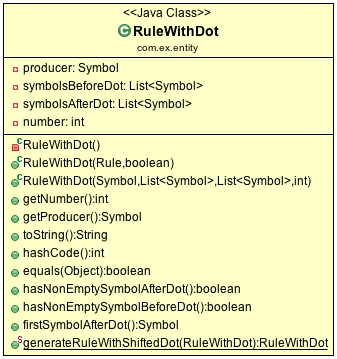
\includegraphics[width=.9\linewidth]{./media/ruleWithDot.png}

O método \texttt{generateRuleWithShiftedDot} serve para gerar um novo objeto do tipo
\texttt{RuleWithDot} com o ponto deslocado para a direita. Usando o exemplo anterior, o
objeto gerado a partir de A \(\rightarrow\) BC.DE representaria A \(\rightarrow\) BCD.E.
Note que o objeto retornado é um novo. Não há efeitos colaterais.

\subsubsection{Ações}
\label{sec:orgheadline11}
Ações no contexto da tabela SLR são representadas por classes.

Além de ter um tipo específico, uma \texttt{Action} contém atributos para indicar sua
posição na tabela, a saber, \texttt{lineToStoreActionInTable} e \texttt{columnToStoreActionInTable}.

Assim, a partir de uma lista de todos os objetos do tipo \texttt{Action} gerados é
possível construir a tabela SLR.

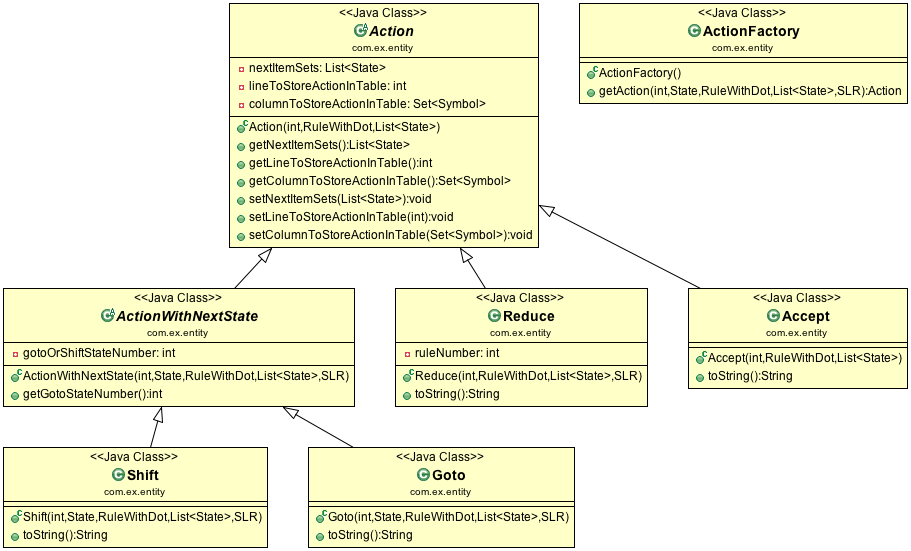
\includegraphics[width=.9\linewidth]{./media/actions.png}

As ações \texttt{Shift} e \texttt{Goto} têm o método \texttt{getGotoStateNumber}, cujo resultado é
armazenado em \texttt{gotoOrShiftStateNumber}.

Esse atributo armazena o número do estado que deve ser usado após executar a
ação. Por exemplo, para um objeto \texttt{Shift} que representa a ação \emph{shift 8}, esse
número é 8. Note que esse número pode indicar um estado que já existe ou um
novo.

Além disso, todas as ações têm um atributo \texttt{nextItemSets} que possui uma lista
de todos os estados descobertos após essa ação. Se a ação é  \texttt{Accept} ou
\texttt{Reduce}, essa lista é exatamente a mesma de antes. Por outro lado, no
caso de \texttt{Shift} e \texttt{Goto}, calcula-se goto(q, a), em que \emph{q} é o estado sendo
analisado e \emph{a} é o primeiro símbolo após o ponto, e se o resultado de goto(q,
a) não estiver na lista de estados conhecida até então, um novo estado é
adicionado a ela. Se o resultado de goto(q, a) já estiver na lista de estados,
então esta permanece a mesma.

O código abaixo ilustra esse processo no caso do \texttt{ActionWithNextState}.

\begin{verbatim}
public ActionWithNextState(int currentStateNumber, State state, RuleWithDot ruleWithDot, List<State> allStates, SLR slr) {
  super(currentStateNumber, ruleWithDot, allStates);
  List<State> newItemSets = new ArrayList<State>();
  newItemSets.addAll(allStates);

  // Sets next state number and the new list of states.
  State nextState = slr.gotoSet(state, ruleWithDot.firstSymbolAfterDot());
  this.gotoOrShiftStateNumber = slr.getStateNumber(nextState, allStates);
  if (gotoOrShiftStateNumber == allStates.size()) {
    newItemSets.add(nextState);
  }
  setNextItemSets(newItemSets);
}
\end{verbatim}

Note que \texttt{newItemSets} é uma \emph{nova} lista de estados. Assim, não há efeitos
colaterais envolvidos.

\subsubsection{Algoritmo}
\label{sec:orgheadline12}
Ainda à maneira do cálculo dos conjuntos anteriores, o algoritmo consiste em adicionar
novos estados à lista de estados até encontrar um ponto fixo. No entanto, a
implementação é um pouco mais complicada, pois o conjunto de estados que estamos
iterando é alterado durante a iteração.

\begin{verbatim}
private final void buildAllItemSets() {
  System.out.println("\n\n\n==============================");
  System.out.println("Building all states.");

  // adding first state
  System.out.println("Adding first state set:");
  List<State> allStatesBeforeIteration = new ArrayList<State>();
  Set<RuleWithDot> firstRuleSet = grammarWithDots.get(grammar.getStartSymbol());
  State firstState = closure(new State(firstRuleSet));
  allStatesBeforeIteration.add(firstState);

  ActionFactory actionFactory = new ActionFactory();

  int indexOfLastStateInWhichAllRulesWereAnalysed = -1;
  boolean setOfAllStatesHasChanged = true;
  while (setOfAllStatesHasChanged) {
    System.out.println("******* New iteration (building all state sets) *******");
    setOfAllStatesHasChanged = false;
    List<State> allStatesAfterIteration = new ArrayList<State>();
    allStatesAfterIteration.addAll(allStatesBeforeIteration);

    for (int currentStateNumber = indexOfLastStateInWhichAllRulesWereAnalysed + 1; currentStateNumber < allStatesBeforeIteration.size(); currentStateNumber++) {
      State state = allStatesAfterIteration.get(currentStateNumber);
      System.out.format("Analysing state %s: %s\n", currentStateNumber, state);
      for (RuleWithDot ruleWithDot : state.getRules()) {
        System.out.println("~~Analysing rule~~");
        System.out.format("Analysing rule: %s\n", ruleWithDot);
        Action act = actionFactory.getAction(currentStateNumber, state, ruleWithDot, allStatesAfterIteration, this);
        this.allActions.add(act);
        System.out.format("\nCreating action: \n %s\n", act);
        System.out.format("Action position:\n Line: %s \n Columns: %s\n\n", act.getLineToStoreActionInTable(), act.getColumnToStoreActionInTable());
        allStatesAfterIteration = act.getNextItemSets();
      }
      indexOfLastStateInWhichAllRulesWereAnalysed++;
    }

    if (allStatesAfterIteration.size() != allStatesBeforeIteration.size()) {
      setOfAllStatesHasChanged = true;
    }

    allStatesBeforeIteration = allStatesAfterIteration;
  }
  System.out.format("All state sets found: %s", allStatesBeforeIteration);
  this.allStates =  allStatesBeforeIteration;
}
\end{verbatim}

O código itera do último estado completamente analisado (isto é, cujas
regras já tiveram as ações correspondentes criadas) até o último estado conhecido.
Para cada item de cada estado é criada uma ação. Um objeto da classe
\texttt{ActionFactory} decide qual é o tipo de ação a ser criada analisando qual é o
símbolo após o ponto. Após a criação da ação, esta tem seu método
\texttt{getNextItemSets} executados, que retorna a nova lista de estados (possivelmente com
um novo estado, se a ação criada for um Shift ou Goto).

\section{Próximos passos}
\label{sec:orgheadline15}
A construção deste programa mostrou-se bastante trabalhosa, e à medida em que o
desenvolvimento avançou, foi possível detectar alguns pontos que ainda podem
melhorar. Listamos a seguir quais seriam os próximos passos para aperfeiçoar o código. 
\begin{itemize}
\item Simplificar o método \texttt{buildAllItemSets}. É possível usar um \texttt{while} em vez de
\texttt{foreach}, de tal forma que não é necessário fazer a distinção entre conjunto
de estados antigo e novo.
\item É fortemente recomendada a inclusão de \texttt{unit tests} para métodos que envolvem
computações importantes nos algoritmos, tornando futuros \emph{refactorings} mais seguros.
\item Buscar utilizar mais métodos de programação funcional introduzidos no Java 8
quando isso tornar o código mais simples.
\end{itemize}
\section{Conclusão}
\label{sec:orgheadline16}
\section{Adendo - notas sobre algumas decisões de \emph{design}}
\label{sec:orgheadline3}
\subsection{Objetos em estados inconsistentes}
\label{sec:orgheadline17}
É desejável que um objeto tenha um estado consitente imediatamente após sua
criação. Em termos prático, isso significa usar seu construtor para setar todos
os atributos necessários. O contrário disso (e, portanto, não recomendado) é não
inserir nada no construtor e depois colocar valores nos atributos através de \emph{setters}. 
Essa prática torna o código menos seguro, pois enquanto todos os atributos não
estão setados, o objeto está num estado inconsistente. Nesse contexto, acessar um
atributo não inicializado retornaria \texttt{null}.

Exemplo de código que segue esse princípio:

\begin{verbatim}
public Grammar(String inputGrammar) throws Exception {
  initialiseOutputMap();

  this.numberOfRules = 0;
  this.rules = new HashMap<Symbol, Set<Rule>>();
  this.terminals = new HashSet<Symbol>();
  this.nonTerminals = new HashSet<Symbol>();

  isValidGrammar(inputGrammar);

  this.startSymbol = addStartSymbol(inputGrammar);
  addNonTerminals(inputGrammar);
  addTerminals(inputGrammar);
  readAllRules(inputGrammar);
  buildAllNonTerminalsThatProduceEps();
  buildAllFirstSets();
  buildAllFollowSets();
  printOutput();
}
\end{verbatim}

\subsection{Minimização de acessibilidade}
\label{sec:orgheadline18}
Classes que não serão estentidas devem ser declaradas como \texttt{final}. O mesmo vale
para métodos que não devem ser sobrescritos.

\begin{verbatim}
// exemplo
public final class Rule {
\end{verbatim}

Os atributos e métodos devem ter a \emph{menor} visibilidade possível. Em
geral, isso significa usar \texttt{private} sempre que possível.

Além disso, é recomendável minimizar o uso de \emph{acessors}. \emph{getters} e \emph{setters}
devem ser adicionados apenas quando necessário. Em vez deles, é preferível criar
métodos que, acessando a informação interna do objeto, retorne o que foi pedido.
Isto está em acordo com o princípio "Tell, Don't Ask". A aplicação desse
princípio mostrou-se difícil para o projeto, pois a interação entre objetos nos
algoritmos depende essencialmente de seus atributos.

\begin{verbatim}
// extraído da classe RuleWithDot

// não há acessor para o atributo symbolsAfterDot,
// pois em momento algum há necessidade de saber isso.
// No entanto, outras classes podem precisar do símbolo após o ponto.
// Elas devem usar o método abaixo.
// O incorreto seria criar um getter para symbolsAfterDot e fazer com
// que as demais classes o usassem, seguidos de get(0).
// Isso violaria o encapsulamento da classe RuleWithDot.
  public Symbol firstSymbolAfterDot() {
    return symbolsAfterDot.get(0);
  }
\end{verbatim}

Este princípio está descrito em Effective Java - Item 13: Minimize the accessibility of classes and members.

\subsection{Minimização de mutabilidade}
\label{sec:orgheadline19}
Algumas classes representam entidades imutáveis. Por exemplos, uma classe \texttt{Coordenada}
que tem um par de inteiros como atributos e que representa uma coordenada deve
ser imutável. Criar um \emph{setter} para esta classe seria absurdo, pois o mesmo
objeto poderia representar uma infinidade de coordenadas diferentes.

Além disso, mutabilidade pode tornar o código complexo e de difícil compreensão.

Identificamos classes que representam entidades imutáveis e nos certificamos que
seus objetos de fato não podem jamais ser alterados. A classe \texttt{Symbol} ilustra
isso bem.

\begin{verbatim}
// classe é marcada como final
 public final class Symbol {

// atributos são privados
  private SymbolType type;
  private String literalRepresentation;

// não há setters
  public Symbol(String literalRepresentation) throws Exception {
    super();
    this.literalRepresentation = literalRepresentation;
    this.type = getType(literalRepresentation);
  }
\end{verbatim}
Este princípio está descrito em Effective Java - Item15: Minimize mutability.

\subsection{Sobrescrever \texttt{hashCode} e \texttt{equals}}
\label{sec:orgheadline20}
Em diversos momentos utilizamos \texttt{equals}. Por exemplo, em \texttt{SLR}, quando 
o conjunto goto de uma ação é calculado, verificamos se o conjunto é igual a algum
estado que já está represente na lista de estados. Para tanto, \texttt{equals} é usado
para comparar objetos da classe \texttt{State}.

Isso só é possível de ser feito de forma correta porque \texttt{hasCode} também foi
sobrescrito. Isso acontece porque ao checar a igualdade de objetos, antes de
de fato executar o código sobrescrito em \texttt{equals}, verifica se os códigos \emph{hash}
dos dois objetos são iguais. Se não são, então a comparação resulta em \texttt{false},
mesmo se todas as condições do \texttt{equals} fossem satisfeitas.

\begin{verbatim}
// extraído da classe Symbol
  @Override
  public int hashCode() {
    final int prime = 31;
    int result = 1;
    result = prime * result + ((literalRepresentation == null) ? 0 : literalRepresentation.hashCode());
    result = prime * result + ((type == null) ? 0 : type.hashCode());
    return result;
  }

  @Override
  public boolean equals(Object obj) {
    if (this == obj)
      return true;
    if (obj == null)
      return false;
    if (getClass() != obj.getClass())
      return false;
    Symbol other = (Symbol) obj;
    if (literalRepresentation == null) {
      if (other.literalRepresentation != null)
        return false;
    } else if (!literalRepresentation.equals(other.literalRepresentation))
      return false;
    if (type != other.type)
      return false;
    return true;
  }
\end{verbatim}

Este princípio está descrito em Effectie Java- Item 9: Always override hashCode when you override equals.

\section{Referências Bibliográficas}
\label{sec:orgheadline21}
\end{document}